\chapter{Methodology}
\section{Fix correctness violation}
    There are two ways to fix the correctness violation mentioned at the last paragraph in the previous chapter. Seeing Figure
~\ref{fig:my_label1}, one is to add barrier between kernels so the next kernel will not start until all work group finish the previous kernel and stored the result into global memory. The other one is to do redundant works, calculating all the data needed itself in every work group.

\begin{figure}[hbtp]
\centering
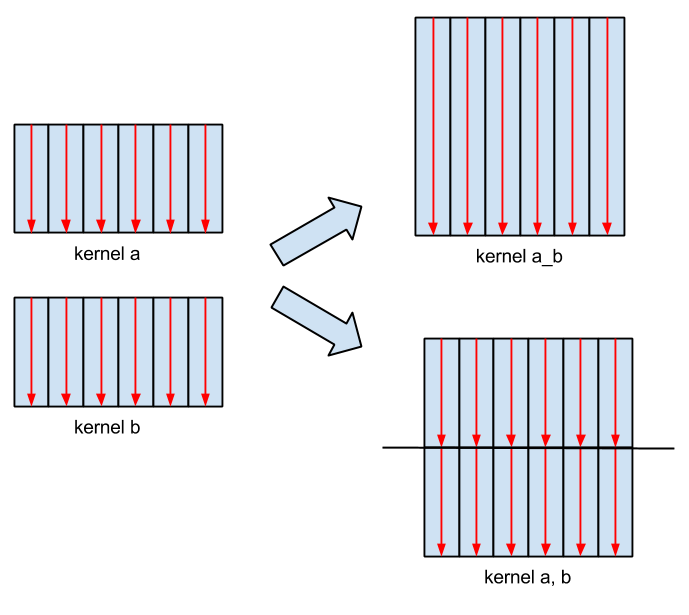
\includegraphics[width=15cm]{img/kernel-fusion.png}
\caption{kernel fusion}
\label{fig:my_label1}
\end{figure}

\section{Halide schedule compute\_at}
    Halide provide a schedule named “compute\_at”, and it can fuse multiple kernels into one kernel. The schedule uses the second way, doing redundant works to calculate the data needed itself. The main disadvantage of this way is, the more the kernels fused, the more the redundant works shows.

    For example, Figure~\ref{fig:my_label2} shows the pixels accessed to calculate one pixel’s result. The pink part represents the pixels accessed in the kernel.The algorithm is to obtain the pixel on the target pixel’s left and right, and calculate the sum of the two pixels and the target pixel. The example shows processing the image using the algorithm two times. We can see every kernel access two extra pixels except the target pixel.
	
\begin{figure}[hbtp]
\centering
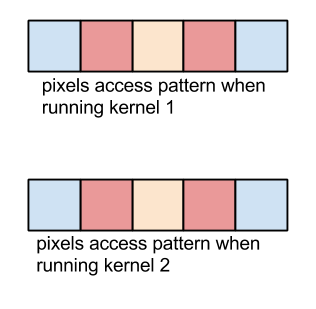
\includegraphics[width=8cm]{img/figure2.png}
\caption{accessing pattern of 2 kernels}
\label{fig:my_label2}
\end{figure}

    Figure~\ref{fig:my_label3} shows the calculating flow of doing one dimension blur algorithm twice, and applying kernel fusion by doing redundant works. We can see the number of pixels accessed are five in the first kernel, and three in the second kernel.
	
\begin{figure}[hbtp]
\centering
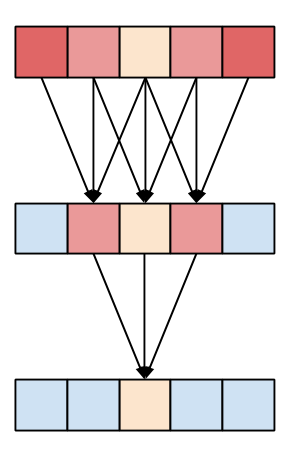
\includegraphics[width=8cm]{img/figure3-6(for-paper).png}
\caption{Example of the calculating flow when doing redundant works}
\label{fig:my_label3}
\end{figure}
	
    Figure~\ref{fig:my_label4} shows the pixels accessed to calculate one pixel’s result if we use Halide schedule, compute\_at. The pink part represents pixels accessed in the first kernel. The burgundy part represents the extra pixels accessed in the second kernel. We can see if we want to eliminate the dependency without barrier, we need to access two extra pixels than original.
	
\begin{figure}[hbtp]
\centering
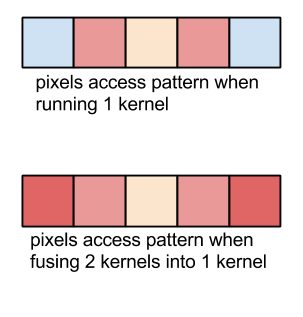
\includegraphics[width=8cm]{img/figure3.png}
\caption{accessing pattern of compute\_at}
\label{fig:my_label4}
\end{figure}
	
    Figure~\ref{fig:my_label5} shows the accessing pattern using kernel fusion when processing an image with a blur algorithm accessing the 8 pixels around the target pixel. The pink part represents pixels accessed in the first kernel. The burgundy part represents the extra pixels accessed in the second kernel. We can see when blurring the image 2 times, the increasing redundant works are to calculate 16 pixels compared to the original version. And the redundant works will be calculating 24 pixels compared to only fuse 2 kernels into one if we fuse 3 kernels into one kernel. So the redundant works grow fast according to how many kernels we fuse.

\begin{figure}[hbtp]
\centering
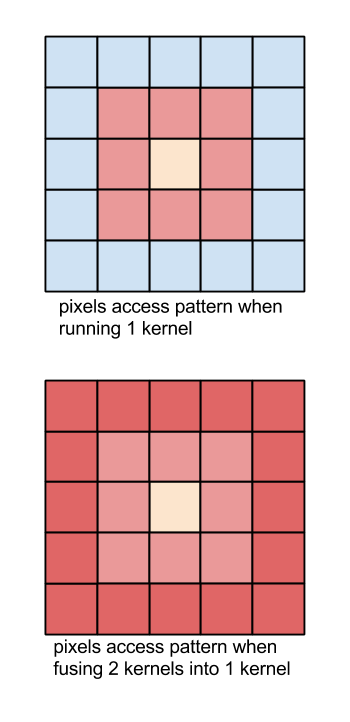
\includegraphics[width=10cm]{img/figure4.png}
\caption{accessing pattern of compute\_at 2}
\label{fig:my_label5}
\end{figure}

\section{Approach: enqueue\_kernel}
    We implement our enqueue\_kernel feature on an Open-Source Project - POCL (Portable Computing Language.) It is an OpenCL implementation. Our approach will help the user to branch to the new kernel at runtime by using the “block” which is defined by the Clang\cite{clangori} (a compiler front end for the C, C++, Objective-C and Objective-C++ programming languages) and it can be used like a function pointer. According to the OpenCL 2.0 spec, enqueue\_kernel’s second input argument is “kernel\_enqueue\_flags\_t flags”. The flags can be CLK\_ENQUEUE\_FLAGS-\_NO\_WAIT, CLK\_ENQUEUE\_FLAGS\_WAIT\_KERNEL and CLK\_ENQUEUE\_FLA-
GS\_WAIT\_WORK\_GROUP.

    Figure~\ref{fig:my_label6} is a flowchart presenting our approach. We implement our approach pre-parser inside the host OpenCL API clCreateProgramWithSource. When the kernel source code are input, our pre-parser will process the source code according to which flag is specified.

    Our approach can perform full functionality of the last flag mentioned, but leave the first and the second flag limited functionality. We add a pre-parser before compiling the kernel source code to binary program (before clCreateProgramWithSource.) to do setup for the enqueue\_kernel function according to the kernel\_enqueue\_flags\_t. 
	
\begin{figure}[hbtp]
\centering
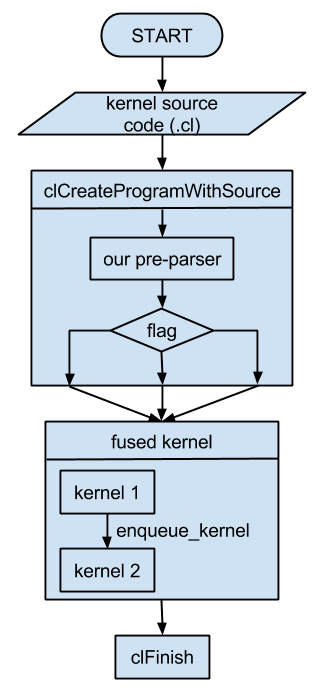
\includegraphics[width=10cm]{img/overview-approach.png}
\caption{Flowchart of approach}
\label{fig:my_label6}
\end{figure}

    If the last flag is specified, we will switch the enqueue command to the last line of the kernel. And then branch to the new kernel using block. This will let all work items within a work group wait for all work items to finish their previous kernel, and then branch to the new kernel by block.
    If the second flag is specified, we will switch the enqueue command to the last line with a barrier before it. But this will not let all work group wait for the others to finish the previous kernel, since synchronization between work groups cannot be done using OpenCL currently.
    If the first flag is specified, we will immediately branch to the new kernel by block. So the current kernel will be blocked and wait for the new kernel to finish. But the full functionality of the first flag should be enqueueing the new kernel, and then create a new thread for the new kernel. So the new kernel and the current kernel can be running at the same time. This will give the process better performance than our approach. But the first flag won’t be used when performing kernel fusion. The new kernel should have no dependency with the original kernel, since they should run at the same time.
	
\section{Comparison between two features}
    Besides Halide schedule “compute\_at” need to do redundant works, while our approach may not need to, one more difference is that our approach supports deciding which kernel to be fused at runtime. This can be used to perform dynamic kernel fusion while Halide schedule “compute\_at” can not. Halide schedule compute\_at need to decide which kernel to be fused at compile time, and Halide CodeGen will generate the corresponding OpenCL host and device source code.

\section{Different Approach: enqueue\_kernel}
    According to the original OpenCL 2.0 spec, there are some more built-in functions, host CL APIs, helper functions and data type definitions that need to be supported. Including host CL APIs clCreateCommandQueueWithProperties, built-in function get\_default\_queue. 
    clCreateCommandQueueWithProperties can be used to create a command queue with different properties supported. Since with different kernel enqueued, we may need command queue with different properties. The properties will be stored as a list. And the get\_default\_queue built-in function will be used to get the default device queue during the kernel (device queue is supposed to be the default command queue, in order to put the new enqueue kernel command into the default command queue.) 
	
    By using the host API clCreateCommandQueueWithProperties and the built-in function get\_default\_queue, we can put the kernel which we want to enqueue in the current kernel into the default command queue which we can obtain from get\_default\_queue and then enqueue it through the OpenCL command queue feature.
	
    But the difficulty here is, according to the OpenCL 2.0 spec, the enqueue\_kernel built-in function’s input argument is “block” which is defined by the Clang\cite{clangori} (a compiler front end for the C, C++, Objective-C and Objective-C++ programming languages.) It can be used like a function pointer, so we can not directly obtain the kernel name mapping to this block. But in POCL, we need to first create the whole program by clCreateProgramWithSource to create the binary. It will be compiled to .bc through LLVM (Low Level Virtual Machine), and then being compiled to .so. To enqueue a kernel, we need its kernel name to search for the code section in the .so file. The enqueue command in the command queue should contain the kernel name, which we currently do not have.
	
\section{Temporary storage allocation}
    To use enqueue\_kernel, we will need to allocate temporary storage. Since the output of the previous kernel will be the input of the next kernel, we need a temporary storage to store these data for the next kernel to read them. The storage type should be declared global, so all work items within all work groups can read it.

    We will need to allocate temporary storage at the host source code, and use allocated temporary storage instead of the original storing destination at the kernel source code.
